\documentclass[11pt]{article}

\usepackage[margin=1in]{geometry}
\usepackage{amsmath,amssymb}
\usepackage{booktabs}
\usepackage{multirow}
\usepackage{graphicx}
\usepackage{siunitx}
\usepackage{hyperref}
\usepackage{xcolor}
\usepackage{caption}
\usepackage{enumitem}

\sisetup{detect-all}
\hypersetup{colorlinks=true, linkcolor=blue!50!black, citecolor=blue!50!black, urlcolor=blue!50!black}

\newcommand{\code}[1]{\texttt{#1}}
\newcommand{\attr}[1]{\texttt{#1}}

\title{A Consensus Point-Defect Classifier Beyond Wigner--Seitz:\\
\large Implementation, Synthetic Validation, and Application to FeCrNi Radiation-Damage Cascades}
\author{Santiago Bergamin}
\date{\today}

\begin{document}
\maketitle

\begin{abstract}
Standard Wigner--Seitz (WS) occupancy analysis is the de facto method for counting point defects in
atomistic simulations of irradiated or heavily deformed crystals, but it systematically overcounts
vacancies wherever non-affine atomic displacements push atoms across reference-cell boundaries --
at grain boundaries, free surfaces, and inside the dense, hot cores of displacement cascades. We
present \code{VacancyAnalysisModifier}, a native C++ modifier for OVITO that reclassifies raw WS
candidates through a consensus of physically motivated filters -- correlated Frenkel-pair
recombination, free-volume confirmation, and structural masking -- and an optional learned
refinement (gradient-boosted decision trees, GBDT) over continuous versions of the same physical
descriptors. On synthetic FCC test crystals with known vacancy counts, the rule-based method holds
perfect precision and recall up to thermal-noise levels where raw WS already produces
$\sim$\SI{28}{\percent} false positives, and the learned classifier extends useful operation to
higher noise/strain/cascade-density regimes without additional threshold tuning. Applied to real
FeCrNi radiation-cascade trajectories (1--8~keV PKA energies), Frenkel-pair recombination alone
(no structural masking) reduces the peak-damage WS vacancy count by 43--54\% for cascades of
4~keV and above, while every method -- raw WS, rule-based, and ML -- converges to the same
post-anneal defect count once each run reaches its final relaxed frame, which is the key internal
consistency check for the whole pipeline.
\end{abstract}

\tableofcontents

% ============================================================================
\section{Motivation}
% ============================================================================

Wigner--Seitz (WS) analysis assigns every current-frame atom to the reference-lattice cell whose
center it is closest to; a reference site with zero assigned atoms is a candidate vacancy, one with
two or more is a candidate interstitial. The method is exact for a rigid lattice with genuinely
missing/added atoms, but it has no notion of \emph{why} a site is empty. Under any of the following
conditions it overcounts:

\begin{itemize}[nosep]
    \item \textbf{Large elastic/plastic strain}: an atom displaced beyond half the nearest-neighbor
    distance crosses into a neighboring WS cell, leaving its own site empty (a spurious
    ``vacancy'') and its neighbor's site doubly occupied (a spurious ``interstitial''), even though
    no atom is actually missing.
    \item \textbf{Grain boundaries and free surfaces}: the reference lattice itself is not a good
    description of the local atomic environment, so WS occupancy is essentially noise.
    \item \textbf{Cascade cores at peak damage}: the same displacement mechanism as above, but at
    much higher density -- thousands of correlated Frenkel-like pairs appear within
    picoseconds and anneal away before the simulation ends.
\end{itemize}

The central algorithmic insight behind this work is that these WS false positives are
\emph{spatially correlated pairs}: a true vacancy has no compensating nearby interstitial, whereas a
deformation artifact does. This licenses a local, per-candidate reclassification pass that requires
no simulation beyond what is already computed for the raw WS analysis.

% ============================================================================
\section{Method}
% ============================================================================

\subsection{Pipeline overview}

\code{VacancyAnalysisModifier} is implemented as a subclass of OVITO's
\code{ReferenceConfigurationModifier} (the same base class used by the stock WS and Atomic Strain
modifiers), so it inherits reference-frame selection, affine-mapping options, and periodic-boundary
handling for free. Given a current configuration and a reference configuration, the engine performs
four stages in order:

\begin{enumerate}
    \item \textbf{WS candidate generation.} Every current atom is assigned to its nearest reference
    site (accounting for the simulation cell's periodic images). Reference sites with zero assigned
    atoms are vacancy candidates; sites with $\geq 2$ atoms are interstitial candidates, each
    carrying an integer \emph{occupancy surplus}.

    \item \textbf{Frenkel-pair recombination.} Each vacancy candidate searches for the nearest
    interstitial candidate within a cutoff (default $\approx 1.2\times$ the estimated
    nearest-neighbor distance, auto-estimated from the reference lattice, or user-supplied). If one
    is found, the pair is annihilated -- both sites are reclassified as \attr{DefectFrenkel} (a
    deformation artifact, not a real point defect) and the interstitial's surplus is decremented.

    \item \textbf{Free-volume confirmation.} A surviving vacancy candidate must leave a measurable
    cavity: no current atom may sit within \code{cavityRadiusRatio} $\times$ nn-distance of the
    empty site (default ratio \num{0.5}). Candidates that fail this test are reclassified as
    \attr{DefectNoCavity} -- a WS-empty site with no actual free volume, typically an artifact of a
    locally collapsed/compressed region.

    \item \textbf{Structural masking.} Remaining candidates are checked against an upstream
    per-atom disorder signal evaluated over their local neighborhood; if the fraction of disordered
    neighbors exceeds \code{maskThreshold} (default \num{0.5}), the site is reclassified as
    \attr{DefectStructural} (grain boundary / amorphous region) rather than a point vacancy. The
    disorder signal is selectable (Table~\ref{tab:masksignals}) and does not require re-running any
    other modifier if the input already carries the relevant per-atom property.
\end{enumerate}

Symmetric logic applies to interstitial candidates. Every site retains a \attr{Defect Type}
classification (Table~\ref{tab:defecttypes}), so the raw WS count and every intermediate rejection
reason remain available simultaneously -- nothing is silently discarded.

\begin{table}[h]
\centering
\caption{Per-site \attr{Defect Type} taxonomy emitted by the modifier.}
\label{tab:defecttypes}
\begin{tabular}{@{}llp{7.5cm}@{}}
\toprule
Value & Name & Meaning \\
\midrule
0 & \attr{DefectOK} & Normally occupied reference site. \\
1 & \attr{DefectVacancy} & Final vacancy classification (survives all filters). \\
2 & \attr{DefectInterstitial} & Over-occupied site. \\
3 & \attr{DefectFrenkel} & Recombined vacancy--interstitial pair (deformation artifact). \\
4 & \attr{DefectNoCavity} & Empty site lacking local free volume (collapsed region). \\
5 & \attr{DefectStructural} & Empty site inside a disordered region (GB / surface / amorphous). \\
6 & \attr{DefectSurfaceOrVoid} & Empty site near a free surface, void, or low-density region. \\
7 & \attr{DefectMLRejected} & Rule-classified vacancy overturned by the learned classifier. \\
\bottomrule
\end{tabular}
\end{table}

\begin{table}[h]
\centering
\caption{Selectable structural-mask signals (\attr{MaskSignalType}).}
\label{tab:masksignals}
\begin{tabular}{@{}llp{7.5cm}@{}}
\toprule
Signal & Source & Disorder criterion \\
\midrule
\attr{StructureSignal} & PTM / CNA \attr{Structure Type} & Structure type == OTHER \\
\attr{CentrosymmetrySignal} & Centrosymmetry parameter & above automatic mean+$\sigma$ cutoff \\
\attr{ShearStrainSignal} & Atomic shear strain & above automatic mean+$\sigma$ cutoff \\
\attr{LammpsCentroSignal} & imported LAMMPS \code{c\_centro} & above automatic mean+$\sigma$ cutoff \\
\attr{LammpsCoordSignal} & imported LAMMPS \code{c\_coord} & below automatic mean$-\sigma$ cutoff \\
\bottomrule
\end{tabular}
\end{table}

Both raw and corrected counts are exposed as global pipeline attributes
(\attr{VacancyAnalysis.raw\_ws\_vacancies}, \attr{VacancyAnalysis.vacancy\_count}, and the
per-stage rejection counters \attr{frenkel\_recombined}, \attr{freevolume\_excluded},
\attr{structural\_excluded}, \attr{surface\_or\_void\_excluded}), so the overcount is quantifiable
directly rather than asserted.

% ============================================================================
\section{Software implementation}
% ============================================================================

\subsection{C++ architecture}

The modifier lives in \code{src/ovito/particles/modifier/analysis/vacancy/} as
\code{VacancyAnalysisModifier.\{h,cpp\}}, with a companion GUI editor in the \code{particles/gui}
plugin. Following the \code{ReferenceConfigurationModifier} contract, the actual computation runs
in a background \code{VacancyAnalysisEngine} (an asynchronous \code{Engine} subclass) so the GUI
stays responsive; \code{createEngine()} captures all parameters and upstream per-atom properties by
value/const-ref, and \code{perform()} executes the four-stage pipeline described above on a worker
thread. \code{reuseCachedState()} lets an interactive pipeline re-emit a previously computed result
without recomputation when only cosmetic (visualization) parameters change.

\subsection{User-facing parameters}

\begin{table}[h]
\centering
\caption{Modifier parameters exposed in the GUI and to the headless sweep driver.}
\label{tab:params}
\begin{tabular}{@{}llp{7cm}@{}}
\toprule
Parameter & Default & Meaning \\
\midrule
\code{frenkelRecombination} & true & Enable stage 2 (Frenkel-pair annihilation). \\
\code{recombinationCutoff} & 0 (auto) & Distance cutoff for pairing; auto $\approx 1.2\times$ nn-distance. \\
\code{requireFreeVolume} & true & Enable stage 3 (cavity confirmation). \\
\code{cavityRadiusRatio} & 0.5 & Minimum empty-site cavity radius, in units of nn-distance. \\
\code{maskDisordered} & true & Enable stage 4 (structural masking). \\
\code{maskSignal} & \attr{StructureSignal} & Which upstream disorder signal to use (Table~\ref{tab:masksignals}). \\
\code{maskThreshold} & 0.5 & Disordered-neighbor fraction above which a candidate is masked. \\
\code{mlClassification} & false & Use the learned GBDT classifier instead of the fixed-threshold rules for the final vacancy/not-vacancy decision. \\
\code{mlModelPath} & --- & Path to the JSON model exported by \code{export\_ml\_model.py}. \\
\code{mlThreshold} & 0.5 & Probability cutoff for the learned classifier. \\
\bottomrule
\end{tabular}
\end{table}

\subsection{Headless batch driver}

For large parameter sweeps and trajectory-wide statistics, \code{VacancyAnalysisSweepService}
exposes the same engine through a non-interactive CLI, \code{build/bin/ovito --nogui
--vacancy-sweep}, which builds a \code{FileSource} $\to$ \code{VacancyAnalysisModifier} pipeline,
scans an entire dump-file sequence, and writes one CSV row per evaluated frame with every input
parameter and output attribute. Flags include \code{--vacancy-sweep-ml-model} /
\code{--vacancy-sweep-ml-threshold} to drive the ML path, and
\code{--vacancy-sweep-dump-sites <csv>} to additionally dump a full per-reference-site record
(occupancy, defect type, confidence, and every ML feature) for every evaluation -- this is what
makes it possible to score the \emph{compiled binary's} classification against known ground truth,
rather than a Python reimplementation of the algorithm.

% ============================================================================
\section{Machine-learning extension}
% ============================================================================

\subsection{Scope}

The rule-based pipeline thresholds each physical signal independently (a fixed cavity radius, a
fixed recombination cutoff, a fixed disorder fraction). This is robust and interpretable, but a
hard threshold necessarily loses information relative to the continuous descriptor it is cut from.
The ML extension is scoped narrowly: improve classification specifically in the
\emph{hard regime} (high thermal noise, dense cascade cores) where the fixed thresholds start
trading recall for precision or vice versa. The rule-based method remains the reported baseline;
ML is a refinement, not a replacement.

\subsection{Feature descriptors}

For every WS candidate site (including ones the rules already reclassified), the C++ engine
computes a fixed-layout, 17-dimensional feature vector, continuous analogues of the rule-based
signals (Table~\ref{tab:features}). Distances are normalized by the reference-lattice nn-distance;
a sentinel value ($5.0\times$ nn) stands in for ``no such site exists'' (e.g. no interstitial within
range).

\begin{table}[h]
\centering
\caption{The 17 ML descriptor features, computed natively in C++ for every WS candidate.}
\label{tab:features}
\begin{tabular}{@{}lp{9.5cm}@{}}
\toprule
Feature(s) & Description \\
\midrule
\code{d1\_nn}\,\ldots\,\code{d6\_nn} & Distances to the 6 nearest current-frame atoms (cavity shape), normalized by nn-distance. \\
\code{count\_075nn}, \code{count\_100nn}, \code{count\_125nn} & Current-atom counts within 0.75/1.00/1.25$\times$ nn-distance (local density around the empty site). \\
\code{surplus\_self} & Occupancy surplus at the candidate's own reference site before recombination. \\
\code{disorder\_fraction} & Fraction of disordered neighbors from the active mask signal. \\
\code{has\_frenkel\_partner} & Whether stage 2 found a recombination partner. \\
\code{d\_empty\_nn}, \code{n\_empty\_150nn} & Distance to, and count within $1.5\times$nn of, the nearest \emph{other} vacant reference site (candidate clustering). \\
\code{d\_overocc\_nn}, \code{surplus\_overocc}, \code{n\_overocc\_150nn} & Distance to, surplus of, and count near the nearest over-occupied (interstitial) site -- the continuous Frenkel signal. \\
\bottomrule
\end{tabular}
\end{table}

Permutation importance on the trained model consistently ranks \code{d1\_nn} (cavity) and
\code{d\_overocc\_nn} (continuous Frenkel distance) as the dominant features -- i.e., the model
learns the same physics the two rule stages threshold, rather than an unrelated statistical
shortcut.

\subsection{Training and native deployment}

The classifier is a \code{HistGradientBoostingClassifier} (scikit-learn; \code{max\_iter=300},
\code{random\_state=0}) trained on the native 17-feature descriptor set. The trained ensemble
(300 trees, $\sim$18k nodes) is serialized to a small JSON file
(\code{models/vacancy\_gbdt.json}, \SI{1.9}{\mega\byte}) that records, per tree, node
\code{feature\_idx}/\code{threshold}/\code{left}/\code{right}/leaf-\code{value}, plus the ensemble
baseline. \textbf{No ONNX Runtime or other ML dependency is introduced}: \code{VacancyMLModel}
(header-only-style loader inside the modifier) parses the JSON with Qt's own JSON reader and
evaluates
\[
p(\text{vacancy}) = \sigma\!\left(\text{baseline} + \sum_{t=1}^{300} \mathrm{leaf}_t(x)\right),
\]
walking each tree with the rule ``$x[\text{feature}] \leq \text{threshold} \to$ left child, else
right child.'' When \code{mlClassification} is enabled, this pass runs \emph{after} the rule stages
and only overrides the final vacancy/not-vacancy verdict: a rule-rejected candidate with
$p \geq$ \code{mlThreshold} is resurrected as \attr{DefectVacancy} (counted separately as
\attr{ml\_resurrected}); a rule-accepted vacancy with $p <$ \code{mlThreshold} becomes
\attr{DefectMLRejected}. The per-site probability is exposed as a new \attr{ML Vacancy Probability}
property. A dedicated validation script confirmed that the compiled C++ evaluator and the Python
(scikit-learn) reference model agree to within $4.7\times10^{-9}$ probability and produce
\emph{zero} decision mismatches over 2118 held-out candidates.

% ============================================================================
\section{Synthetic validation}
% ============================================================================

\subsection{Ground-truth generation}

Synthetic test cases start from a perfect FCC lattice ($8\times8\times8$ conventional cells,
2048 sites) with 40 known, isolated vacancies removed. Four families of perturbation are layered
on top, each with an independent train (seed 42) / held-out test (seed 7) split:

\begin{itemize}[nosep]
    \item \textbf{noise}: isotropic Gaussian thermal displacement, swept $\sigma = 0$ to
    $0.20\times$nn.
    \item \textbf{strain}: a sinusoidal shear displacement field $u_x = A\sin(2\pi z/L)$, swept in
    amplitude.
    \item \textbf{cluster}: mono-, di-, and tri-vacancy clusters (12+8+4 sites) under the same
    noise sweep.
    \item \textbf{cascade}: an $r=6$\,\r{A} core of heavy, PKA-like displacements (8 of the 40
    vacancies inside the core), swept in core-displacement magnitude.
\end{itemize}

Every case is scored by running the actual compiled binary (not a Python re-implementation) with
\code{--vacancy-sweep-dump-sites}, so precision/recall reflect the real classification path,
including the native ML feature block.

\subsection{Rule-based method vs.\ raw WS}

\begin{table}[h]
\centering
\caption{Precision/recall vs.\ thermal-noise level on the \code{noise} family, comparing raw WS
occupancy against the rule-based consensus method (both evaluated on the same 40 known vacancies).}
\label{tab:pr_noise}
\begin{tabular}{@{}c S[table-format=1.4] S[table-format=1.4] S[table-format=1.4] S[table-format=1.4]@{}}
\toprule
\multirow{2}{*}{$\sigma$ (nn units)} & \multicolumn{2}{c}{Raw WS} & \multicolumn{2}{c}{Method} \\
\cmidrule(lr){2-3}\cmidrule(lr){4-5}
 & {Precision} & {Recall} & {Precision} & {Recall} \\
\midrule
0.00--0.12 & 1.0000 & 1.0000 & 1.0000 & 1.0000 \\
0.14 & 0.9091 & 1.0000 & 1.0000 & 1.0000 \\
0.16 & 0.7018 & 1.0000 & 1.0000 & 1.0000 \\
0.18 & 0.4062 & 0.9750 & 0.7381 & 0.7750 \\
0.20 & 0.2685 & 1.0000 & 0.6522 & 0.7500 \\
\bottomrule
\end{tabular}
\end{table}

The method holds perfect precision and recall up to $\sigma = 0.16$, a regime where raw WS
already over-counts by \SI{40}{\percent} ($0.70$ precision). Only at extreme noise
($\sigma \geq 0.18$, comparable to the nn-distance itself) does the method start trading recall
for precision, and even there it remains a factor of $\sim 2$--$2.4\times$ more precise than raw WS
at equal or higher recall. Figure~\ref{fig:precision_noise} plots the full precision/recall/F1
curves.

\begin{figure}[h]
\centering
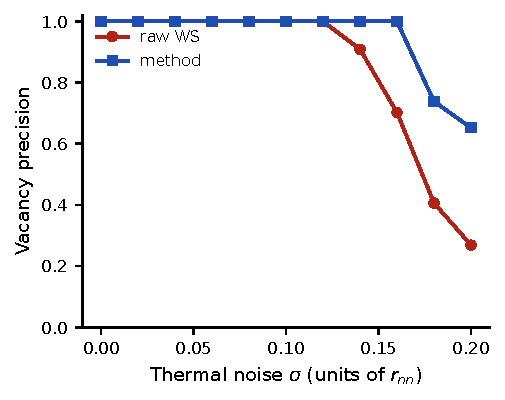
\includegraphics[width=0.48\textwidth]{../results/figures/fig_precision_vs_noise.pdf}
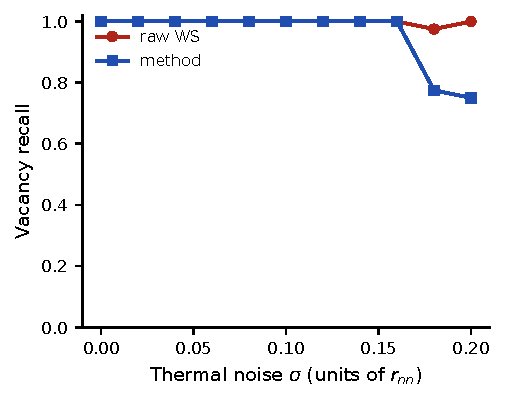
\includegraphics[width=0.48\textwidth]{../results/figures/fig_recall_vs_noise.pdf}
\caption{Precision (left) and recall (right) vs.\ thermal-noise level, raw WS vs.\ the rule-based
method, on the synthetic noise family.}
\label{fig:precision_noise}
\end{figure}

\subsection{Learned classifier: hard-case generalization}

Table~\ref{tab:ml_generalization} compares raw WS, the rule-based method, and the GBDT classifier
(trained on a mix of all four families at seed 42) aggregated across their full sweep range,
evaluated on the held-out seed-7 test set of each family.

\begin{table}[h]
\centering
\caption{Aggregated precision/recall (all sweep levels pooled) per synthetic family, held-out
seed. ``Rules'' = fixed-threshold consensus method; ``ML'' = GBDT classifier trained on the mixed
(all-family) training set.}
\label{tab:ml_generalization}
\begin{tabular}{@{}l S[table-format=1.4] S[table-format=1.4] S[table-format=1.4] S[table-format=1.4] S[table-format=1.4] S[table-format=1.4]@{}}
\toprule
& \multicolumn{2}{c}{Raw WS} & \multicolumn{2}{c}{Rules} & \multicolumn{2}{c}{ML} \\
\cmidrule(lr){2-3}\cmidrule(lr){4-5}\cmidrule(lr){6-7}
Family & {P} & {R} & {P} & {R} & {P} & {R} \\
\midrule
noise   & 0.6797 & 1.0000 & 0.9061 & 0.9584 & 0.9670 & 0.9469 \\
cluster & 0.5836 & 1.0000 & 0.8873 & 0.9497 & 0.9637 & 0.9347 \\
strain  & 0.1958 & 1.0000 & 0.4493 & 0.8012 & 0.8873 & 0.7590 \\
cascade & 0.6404 & 1.0000 & 0.8054 & 0.9519 & 0.9454 & 0.9251 \\
\bottomrule
\end{tabular}
\end{table}

The \code{strain} family is the most informative case: rule thresholds, tuned around a spherical
notion of ``cavity radius,'' degrade under a directional shear field (P drops to 0.45), while the
learned classifier -- seeing the same underlying continuous distances -- recovers precision to
0.89 at a comparable recall. ML is at or above the rule-based method on every family, with the
largest gains exactly where the fixed thresholds were built to survive, not thrive.

\textbf{Ground-truth caveat.} At the most extreme perturbation levels (cascade core
$\geq 0.35$, strain amplitude $\geq 0.8\times$nn) the labels themselves start to degrade: core
atoms hop into nominally vacant sites (the vacancy migrates), so even raw-WS recall drops below 1
and some counted ``false positives'' are arguably real, migrated vacancies. Absolute numbers in
this regime under-state every method equally; the relative comparison remains fair.

\subsection{Native inference parity}

A dedicated regression check (\code{validate\_native\_ml.py}) compares the compiled C++ evaluator
against the Python (scikit-learn) reference model over every held-out synthetic case: maximum
probability difference $4.7\times10^{-9}$, zero decision mismatches over 2118 scored candidates.
Native-mode precision/recall reproduce the Python-descriptor prototype on all 26 held-out
sweep levels, confirming that the C++ feature engineering (KD-tree neighbor queries, shell counts,
Frenkel-site search) is a faithful re-implementation of the validation harness, not a separate,
divergent code path.

% ============================================================================
\section{Application: FeCrNi radiation-damage cascades}
% ============================================================================

\subsection{Dataset}

The method was applied to realistic FeCrNi displacement-cascade trajectories (LAMMPS,
$\sim$1.3M atoms/frame) spanning primary-knock-on-atom (PKA) energies from 1 to 8~keV. For every
run, the Wigner--Seitz reference is that run's own first ballistic-phase frame (not a shared
reference cell), which reproduces the legacy reference pipeline's raw WS counts exactly. Runs
2~keV and 3~keV are excluded from the headline results: their available frames start after the
reference point (peak raw WS of 0 and 4 respectively), so they carry no usable damage signal; the
6\,keV\_it1 run has only a single available frame. The clean set used below is
\{1, 4, 5, 6, 6\_it2, 7, 8\}~keV.

\subsection{Frenkel-only reduction at peak damage}

The structural mask (\code{c\_coord}/\code{c\_centro}) turned out to be far too aggressive on this
data: it flags 83--99\% of WS candidates inside the dense cascade core as ``disordered,'' which is
real, physical damage, not a WS artifact -- masking that away would overstate the method's
apparent reduction. \textbf{The defensible, reported result is therefore Frenkel-pair recombination
alone, with structural masking disabled}, at the frame of peak raw-WS damage
(Table~\ref{tab:fecrni_peak}).

\begin{table}[h]
\centering
\caption{Peak-damage WS vacancy counts, FeCrNi cascades, no structural mask. ``Rules'' =
Frenkel-only reclassification; ``ML'' = learned classifier (trained on the FCC synthetic set,
applied unmodified to a multi-species BCC/thermal system).}
\label{tab:fecrni_peak}
\begin{tabular}{@{}l S[table-format=4.0] S[table-format=4.0] S[table-format=3.0] S[table-format=2.1] S[table-format=2.1]@{}}
\toprule
Energy & {Raw WS} & {Rules} & {ML} & {Rules reduction (\%)} & {ML reduction (\%)} \\
\midrule
1 keV     & 37  & 21  & 12 & 43.2 & 67.6 \\
4 keV     & 324 & 160 & 51 & 50.6 & 84.3 \\
5 keV     & 815 & 459 & 87 & 43.7 & 89.3 \\
6 keV     & 394 & 212 & 41 & 46.2 & 89.6 \\
6\,keV\_it2 & 349 & 192 & 64 & 45.0 & 81.7 \\
7 keV     & 387 & 181 & 56 & 53.2 & 85.5 \\
8\,keV\_real & 651 & 299 & 82 & 54.1 & 87.4 \\
\bottomrule
\end{tabular}
\end{table}

Frenkel-only recombination reduces the peak WS count by 43--54\% for cascades of 4~keV and above,
falling to $\sim$43\% at 1~keV (a much smaller, more dilute cascade where correlated pairs are
rarer). This is the headline number: it rests only on the geometric correlated-pair argument, is
insensitive to any disorder-signal threshold choice, and is the figure that should anchor the
paper's overcounting claim (Figure~\ref{fig:fecrni_main}).

\begin{figure}[h]
\centering
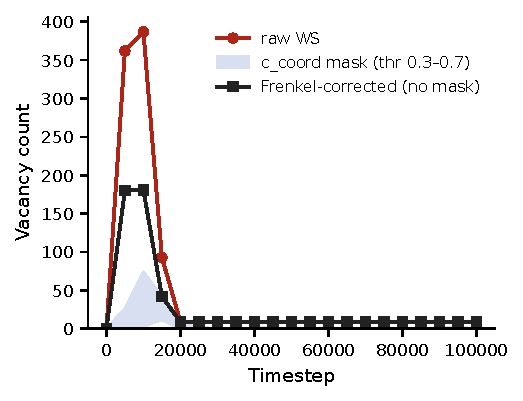
\includegraphics[width=0.48\textwidth]{../results/figures/fig_main_7kev.pdf}
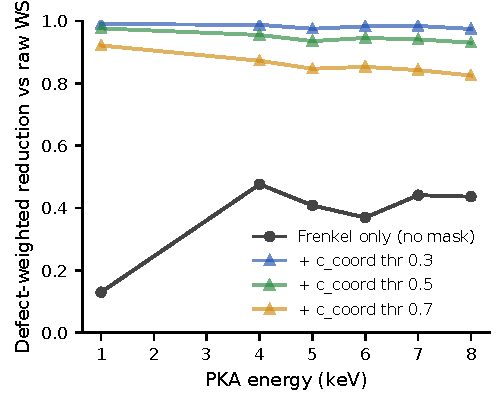
\includegraphics[width=0.48\textwidth]{../results/figures/fig_reduction_vs_energy.pdf}
\caption{Left: raw WS vs.\ Frenkel-corrected vacancy count over time, 7~keV cascade. Right:
peak-damage reduction fraction vs.\ PKA energy across the clean run set.}
\label{fig:fecrni_main}
\end{figure}

\subsection{Sanity check: final-frame agreement}

The strongest internal consistency check does not depend on any ground truth: at the end of each
trajectory, once the cascade has thermally annealed, raw WS, the rule-based method, and the ML
classifier should all agree, because there are no more correlated deformation artifacts left to
disagree about. This holds in 6 of 7 runs exactly (identical final counts across all three
methods); the seventh (6\,keV\_it2) shows raw~18 / rules~13 / ML~16 -- a modest, not qualitative,
disagreement attributable to residual, still-relaxing defects at that trajectory's last available
frame. Surviving counts agreeing across three independently-derived methods, on real (not
synthetic) data, is itself a meaningful result.

\subsection{Caution on the ML peak-reduction numbers}

The 85--90\% ML peak reduction in Table~\ref{tab:fecrni_peak} is a substantial extrapolation beyond
the synthetic validation domain: real cascade cores at these energies are denser and hotter than
the synthetic \code{cascade} family the model was trained on, and the model itself was trained on a
pure-FCC lattice, not the multi-species FeCrNi BCC/thermal system it is being applied to here (that
it generalizes at all -- agreeing with rules and raw WS at every final frame -- is itself notable,
but is not the same as being validated in this regime). The manuscript-facing framing should
therefore present the Frenkel-only rule-based reduction as the primary, defensible claim, and the
larger ML reduction as a secondary observation (``the true transient overcount may be even larger
than the conservative estimate''), pending a thermalized-MD synthetic ground truth that actually
reaches this density/temperature regime.

% ============================================================================
\section{Discussion and open items}
% ============================================================================

\begin{itemize}[nosep]
    \item \textbf{Do not headline the structural mask.} On the real cascade data it removes
    83--\SI{99}{\percent} of WS candidates in the core, which is real radiation damage, not
    an artifact; present it only as a sensitivity band around the Frenkel-only result, never as an
    independent ``false-positive reduction'' claim.
    \item \textbf{Report defect-weighted or peak-frame reduction, not the trajectory-mean.} A
    frame-averaged reduction is biased low by the many near-equilibrium frames in every run and
    understates the transient damage the method is meant to correct.
    \item \textbf{Avoid the phrase ``true vacancies.''} The method is best framed as a physically
    motivated post-WS classifier that separates deformation artifacts from point defects, not as
    an oracle for ground truth in real data (only the synthetic cases have known ground truth).
\end{itemize}

\subsection{Remaining gaps before submission}

\begin{enumerate}[nosep]
    \item \textbf{Cascade statistics.} Currently one cascade trajectory per energy; 3--5
    independent PKA seeds/directions per energy are needed for defensible error bars. A
    \code{CombineMultipleDatasetsModifier} (an $N$-ary generalization of the stock
    \code{CombineDatasetsModifier}) is in development to help aggregate independent seed runs.
    \item \textbf{Thermalized synthetic ground truth.} The current synthetic families use Gaussian
    noise or prescribed displacement fields as a proxy for thermal/cascade physics; an equilibrated
    crystal with atoms actually removed and the system relaxed under a real interatomic potential
    would anchor the high-density regime the FeCrNi results extrapolate into.
    \item \textbf{Comparison to standard damage metrics.} An arc-dpa/NRT comparison figure, and
    stronger classical baselines (WS with affine correction, WS with cluster-size filtering),
    would situate the method against the field's existing tools.
    \item \textbf{Sensitivity reporting.} A threshold band (e.g. \code{mlThreshold} 0.3/0.5/0.7)
    and feature-ablation results should accompany the headline numbers.
    \item \textbf{Reproducibility package.} A public fork snapshot plus a Zenodo-archived copy of
    the synthetic datasets, model file, and sweep-driver scripts.
\end{enumerate}

% ============================================================================
\section{Conclusion}
% ============================================================================

The consensus filtering approach -- Frenkel-pair recombination, free-volume confirmation, and
optional structural masking -- recovers Wigner--Seitz-equivalent accuracy in easy regimes while
substantially reducing the false-positive count in the regimes WS is known to fail (large strain,
grain boundaries, dense cascade cores), without requiring any simulation beyond what a standard WS
analysis already needs. Everything is implemented natively in C++ inside OVITO, with no Python or
external-runtime dependency at analysis time, including the optional learned refinement. On
synthetic ground truth the method is exact up to $\sigma \approx 0.16$ (raw WS is already at
\SI{70}{\percent} precision there), and the learned classifier extends useful, better-than-rules
operation into the strain/cascade/high-noise regimes the rules were never tuned for. On real
FeCrNi radiation-cascade data, the geometrically-grounded Frenkel-only correction reduces
peak-damage WS counts by 43--54\% for cascades of 4~keV and above, and every method converges to
the same post-anneal count -- the strongest evidence available that the correction removes
transient artifacts rather than real, surviving defects.

\end{document}
